\documentclass{article}
\usepackage[utf8]{inputenc}
\usepackage{subfig}
\usepackage{amsmath}

\usepackage{graphicx}
\usepackage[legalpaper, portrait, margin=0.5cm]{geometry}
% \renewcommand{\thesubfigure}{\roman{subfigure}}

\thispagestyle{empty}
\begin{document}

\begin{figure}[h]
    \centering
    % \subfloat[intensity]{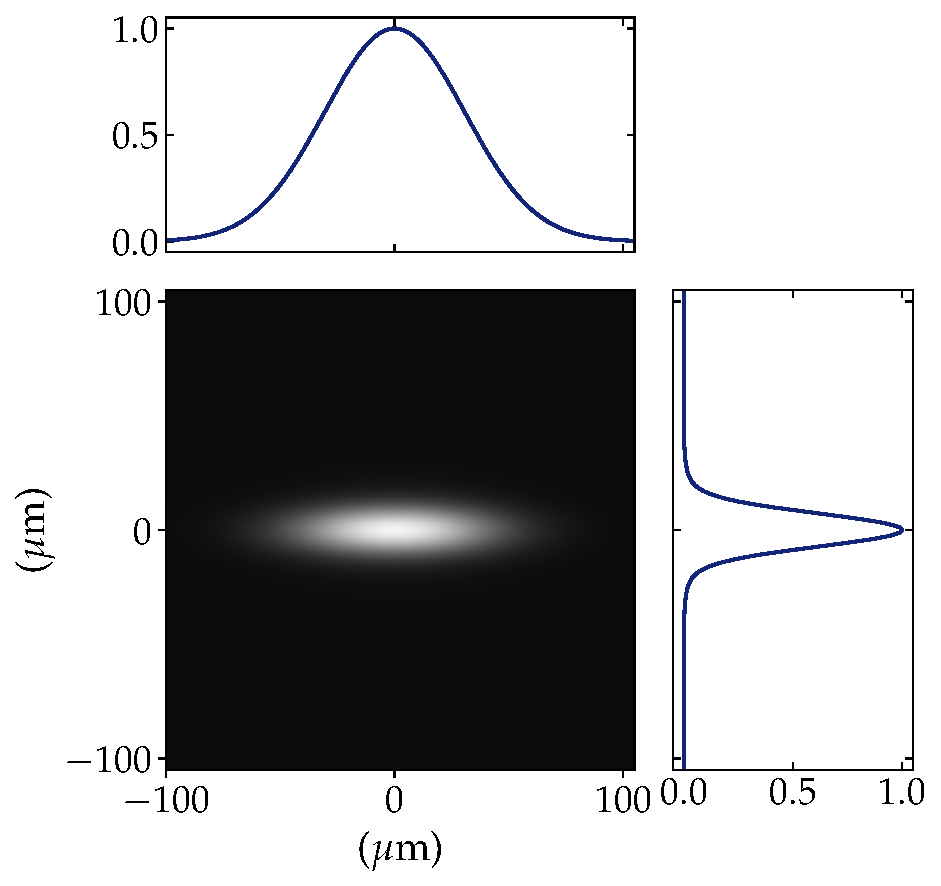
\includegraphics[height=5cm]{figures/CSD_source/intensity_MEconv_7keV.pdf}}\\
    % \subfloat[CSD$_x$]{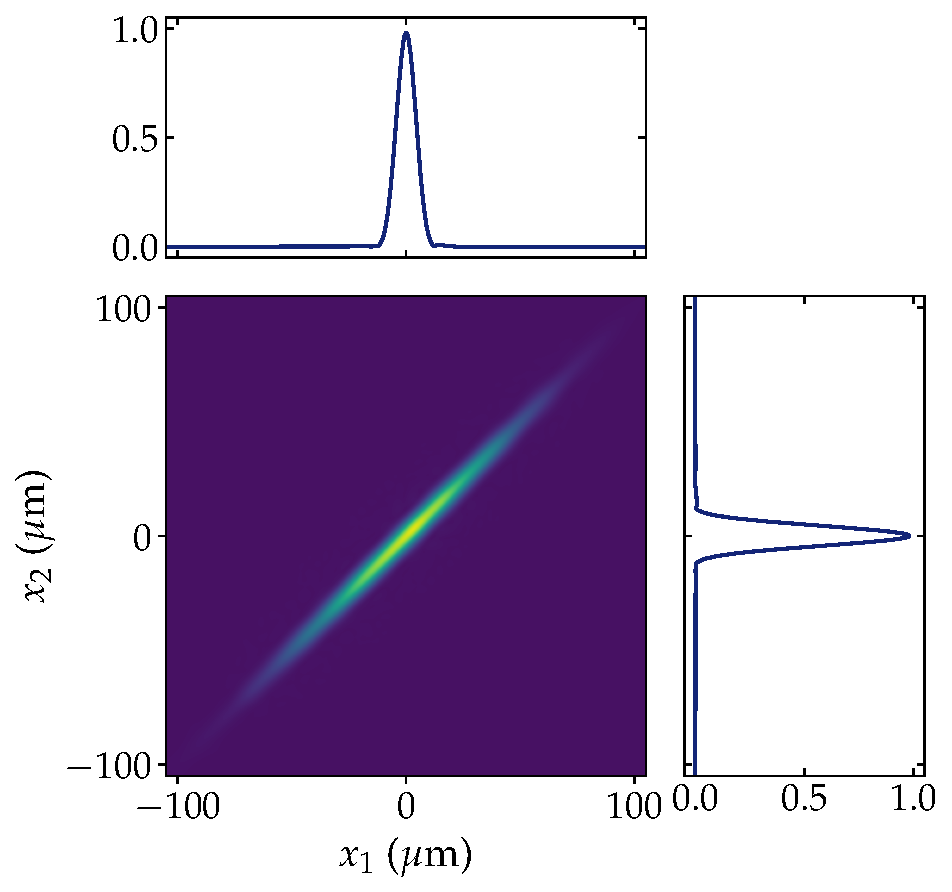
\includegraphics[height=5cm]{figures/CSD_source/CSDx_15kME_7keV.pdf}}\hspace{0.2cm}
    % \subfloat[DoC$_x$]{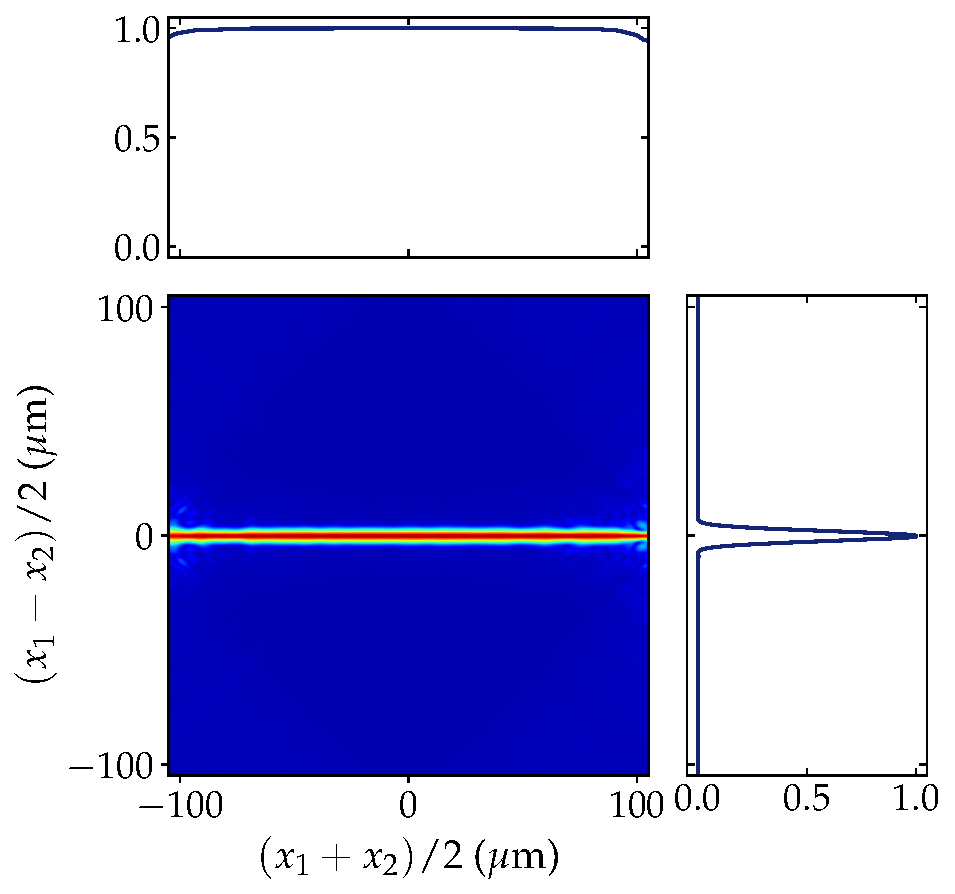
\includegraphics[height=5cm]{figures/CSD_source/DoCx_15kME_7keV.pdf}}\\
    % \subfloat[CSD$_y$]{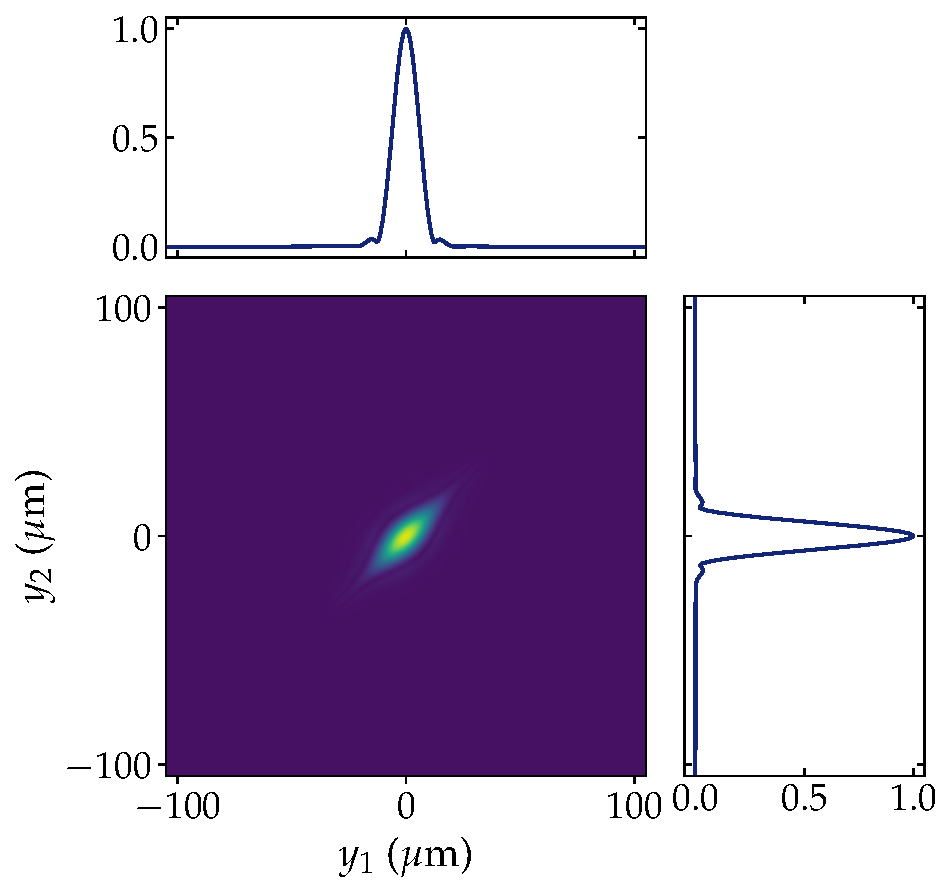
\includegraphics[height=5cm]{figures/CSD_source/CSDy_15kME_7keV.pdf}}\hspace{0.2cm}
    % \subfloat[DoC$_y$]{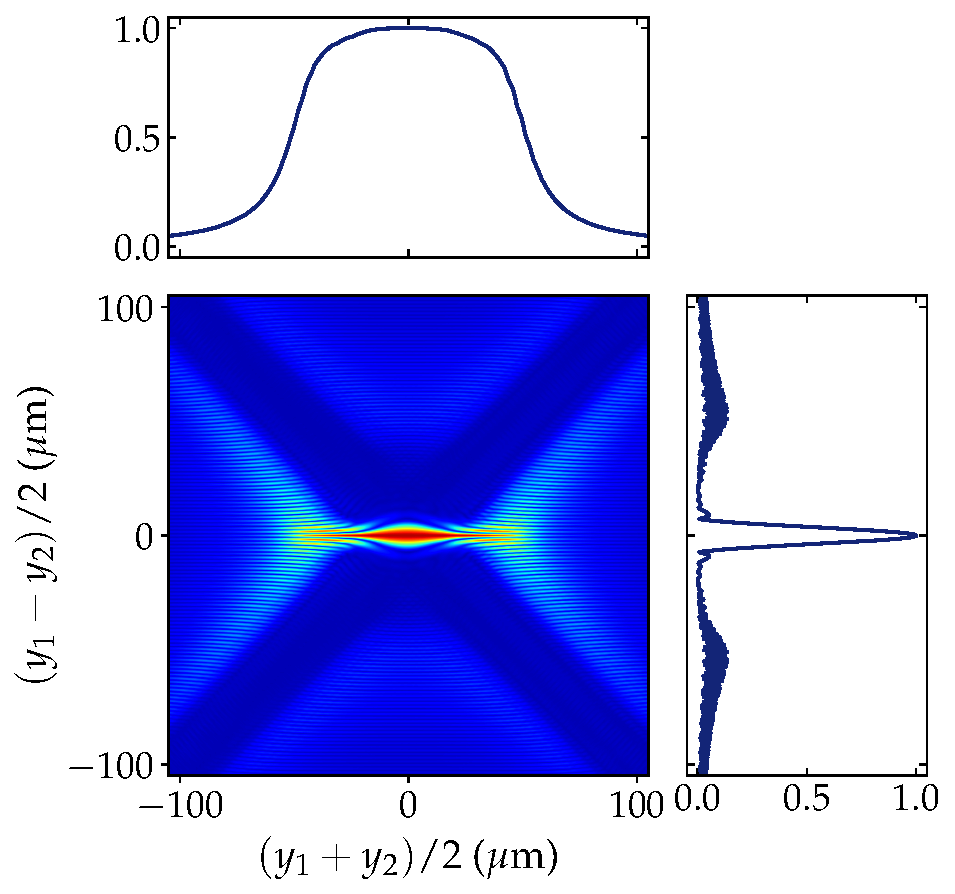
\includegraphics[height=5cm]{figures/CSD_source/DoCy_15kME_7keV.pdf}}\\
    \subfloat[]{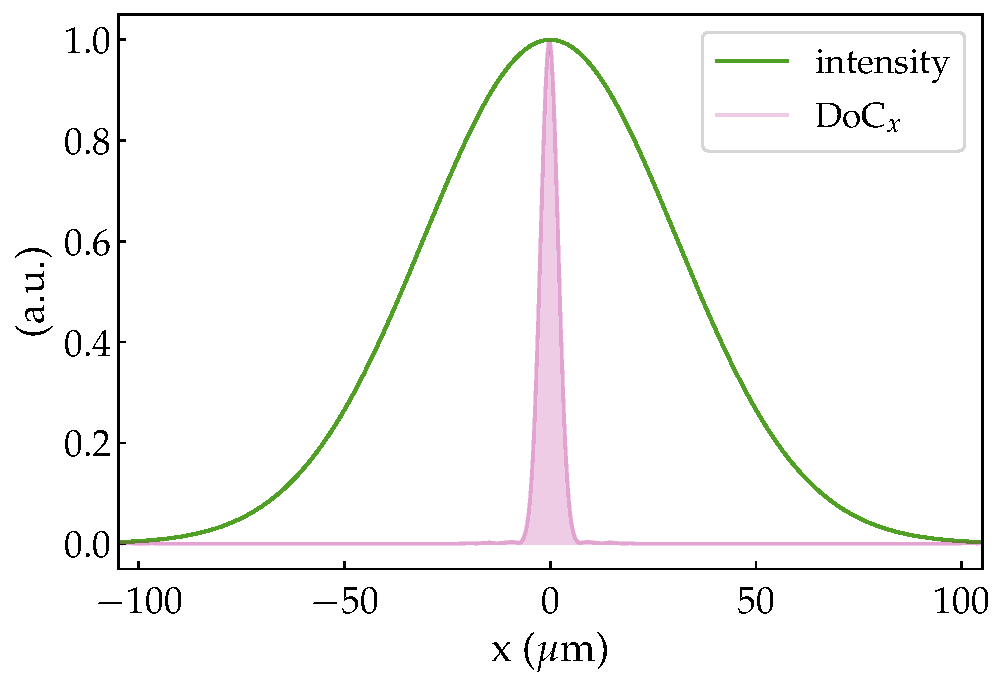
\includegraphics[height=3.5cm]{figures/CSD_source/Ih_vsDoCx_15kME_7keV.pdf}}\hspace{0.2cm}
    \subfloat[]{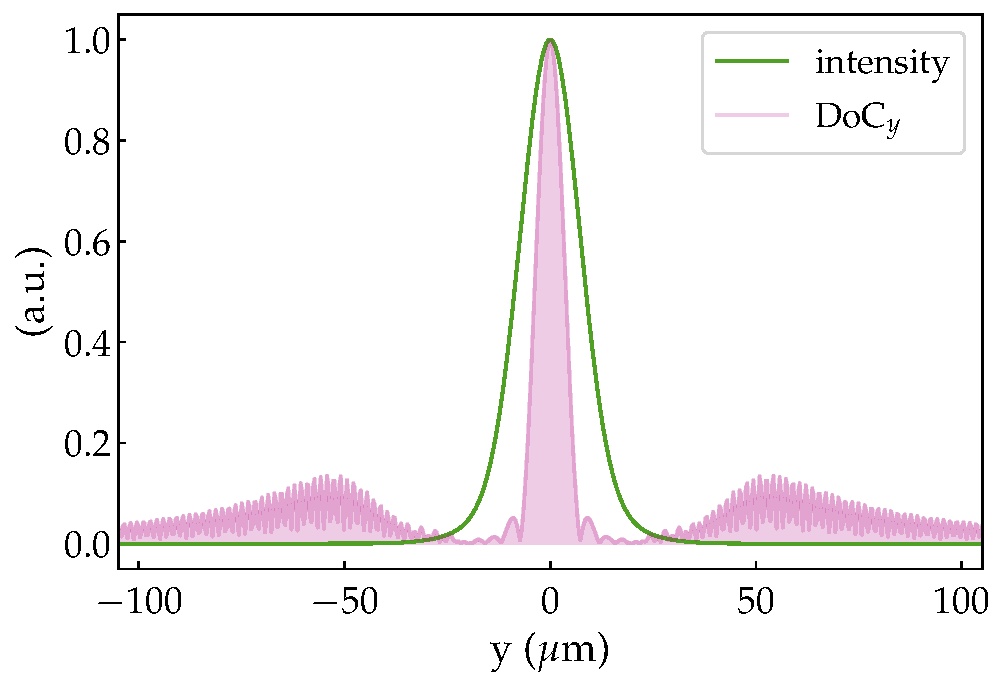
\includegraphics[height=3.5cm]{figures/CSD_source/Iv_vsDoCy_15kME_7keV.pdf}}\\
\end{figure}
\end{document}
